\section{Method}
\label{sec:method}
\begin{figure*}[t]
    \centering
    
\includegraphics[width=0.8\linewidth]{figs/pipeline_new_2.pdf}
    \caption{Overview of the SAGE framework. The main path (black arrows) keeps the original forward flow through Backbone 1 and Backbone 2, with multi-scale skip connections to the decoder. In parallel, the expert path (brown arrows) routes features from an intermediate layer to a sparse expert set (illustrated with Stage~2, Expert~$k$) selected by the router. The Shape-Adapting Hub performs bidirectional format alignment via $S_{\text{in}}$ and $S_{\text{out}}$ so that cross-backbone expert execution is shape-compatible before fusion with the main branch. Blue arrows indicate input/output shape constraints used by the adapters, and dashed boxes denote parameter sharing (expert upcycling from pretrained backbone blocks).}
    \label{fig:main-pipeline}
\end{figure*}

Modern hybrid CNN-Transformer architectures generally depend on static computation graphs, applying the same sequence of operations to all inputs regardless of structural intricacy. While this design is stable and easy to implement, it limits adaptability toward heterogeneous visual patterns. To tackle this limitation, Shape-Adapting Gated Experts (SAGE) reparameterizes a fixed backbone into a two-path architecture with conditional expert routing, as illustrated in Figure~\ref{fig:main-pipeline}. This framework preserves the original backbone pathway while introducing sparse expert selection for feature optimization. The Sparse Mixture-of-Experts formulation is introduced in Section~\ref{subsec:preliminaries_moe}; the SAGE block and hierarchical routing are then detailed in Section~\ref{subsec:sage_block_archi} and ~\ref{subsec:hier_routing}. Finally, Section~\ref{subsec:sahub} presents the Shape-Adapting Hub for cross-architecture feature adaptation and integration.


\subsection{Preliminaries: Sparse Mixture-of-Experts}
\label{subsec:preliminaries_moe}
Our SAGE framework is rooted in the Sparse Mixture-of-Experts (SMoE) formulation~\cite{sparseMoE}, which increases capacity by selectively activating only a subset of expert subnetworks, keeping computation roughly constant. A standard SMoE layer comprises a \textit{router} and a set of experts $\{E_j\}_{j=1}^{M}$. Given an input $x$, the SMoE output is the gated mixture
\begin{equation}
y = \sum_{j \in \mathcal{K}} G(x)_j \, E_j(x),
\label{eq:moe_output}
\end{equation}
where $\mathcal{K}$ is the index set of selected experts. There are multiple choices for implementing $G(x)$, but a simple and performant option is to apply a softmax over the Top-$K$ logits of a linear layer, $G(x) := \text{Softmax}(\text{TopK}(x \cdot W_g))$, so only the chosen experts are evaluated. 

During training, a common issue known as \textit{router collapse} arises when only a few experts dominate the routing. 
To promote balanced utilization, an auxiliary \textit{load-balancing loss} encourages uniform token distribution across experts:
\begin{equation}
\mathcal{L}_{\text{load-balancing}} = M \cdot \sum_{j=1}^{M} f_j \, P_j,
\label{eq:balance_loss}
\end{equation}
where $M$ is the total number of experts, $f_j$ denotes the proportion of tokens distributed to expert $j$ and $P_j$ is the proportion of the gating probability assigned to expert $j$. 

Despite its scalability advantages, conventional SMoE primarily decides \emph{which experts} to activate in a single routing stage.
However, many complex tasks require not only expert selection but also adaptive coordination across heterogeneous computation types.
Motivated by this limitation, our SAGE framework generalizes SMoE by introducing hierarchical routing and heterogeneous expert coordination, enabling the model to adaptively determine both \emph{who} computes and \emph{how} computation is performed for each input.


\subsection{SAGE Block Architecture}
\label{subsec:sage_block_archi}
At each backbone layer $i$ (Figure~\ref{fig:main-pipeline}), SAGE replaces a single deterministic transformation with a \emph{dual-path} block that preserves the original computation while enabling learnable refinement. Given an input feature map $\mathbf{z}_{i-1}$, we compute a baseline feature via the original backbone layer and an enriched feature via sparsely activated layer experts, and then fuse them with a learnable gate.

% \vspace{0.1in}
\noindent\textbf{Main path (backbone preservation).}
The main branch applies the original transformation $f_i(\cdot)$ to obtain a stable baseline feature, $\mathbf{z}_i^{(\text{main})} = f_i(\mathbf{z}_{i-1})$.
This pathway anchors optimization and retains the inductive bias and pretrained initialization of the CNN/Transformer backbone.

% \vspace{0.1in}
\noindent\textbf{Expert path (conditional refinement).}
In parallel, the same input is routed to a sparse set of experts. Following MoLEx-style sparse upcycling~\cite{molex}, experts are the pre-trained backbone layers themselves and their parameters are reused rather than replicated; the router activates only a small subset per input. A hierarchical router (Section~\ref{subsec:hier_routing}) performs top-$K$ selection and yields expert weights $\{w_k\}_{k\in\mathcal{K}}$, while the expert-path feature is formed by weighted aggregation into $\mathbf{z}_i^{(\text{expert})}$. The exact construction of $\mathbf{z}_i^{(\text{expert})}$, including shape-adaptive translation and aggregation, is detailed in Section~\ref{subsec:sahub} and Equations~\ref{eq:sahub_in}--\ref{eq:expert_output}. 

% \vspace{0.1in}
\noindent\textbf{Adaptive fusion.}
We gate between the baseline and expert-refined features using a learnable scalar $\alpha_i$:
\begin{equation}
    \mathbf{z}_i = \alpha_i \cdot \mathbf{z}_i^{(\text{main})} + (1 - \alpha_i) \cdot \mathbf{z}_i^{(\text{expert})},
    \label{eq:combination}
\end{equation}
where $\alpha_i = \sigma(\theta_i)$ is computed from a learnable parameter $\theta_i$. This formulation allows the model to dynamically balance stability and adaptability, favoring expert-driven refinement when beneficial while preserving the backbone's inductive biases when necessary.

% \vspace{0.1in}
\noindent\textbf{Expert pool composition.}
All expert paths draw from a global pool $\mathcal{E}$ with a predefined number of fine-grained experts and shared experts. Both types are implemented as reused backbone layers, but they serve different objectives: fine-grained experts $\mathcal{E}_{\text{fine}}$ focus on depth-specific specialization, whereas shared experts $\mathcal{E}_{\text{shared}}$ encourage domain-generalizable computation. 
% The routing process computes the shared gate $g_s$, computes base logits $\mathbf{L}_i$, modulates them into $\mathbf{L}'_i$, and then applies top-$K$ selection on $\mathbf{L}'_i$. A higher $g_s$ increases the likelihood of selecting shared experts, while a lower $g_s$ biases selection toward fine-grained experts. Unlike always-on shared-expert designs, shared experts in SAGE are also conditionally routed; however, because generalization is broadly beneficial, they are typically selected frequently in practice.

\subsection{Hierarchical Expert Routing}
\label{subsec:hier_routing}

\begin{figure}[t]
    \centering    
    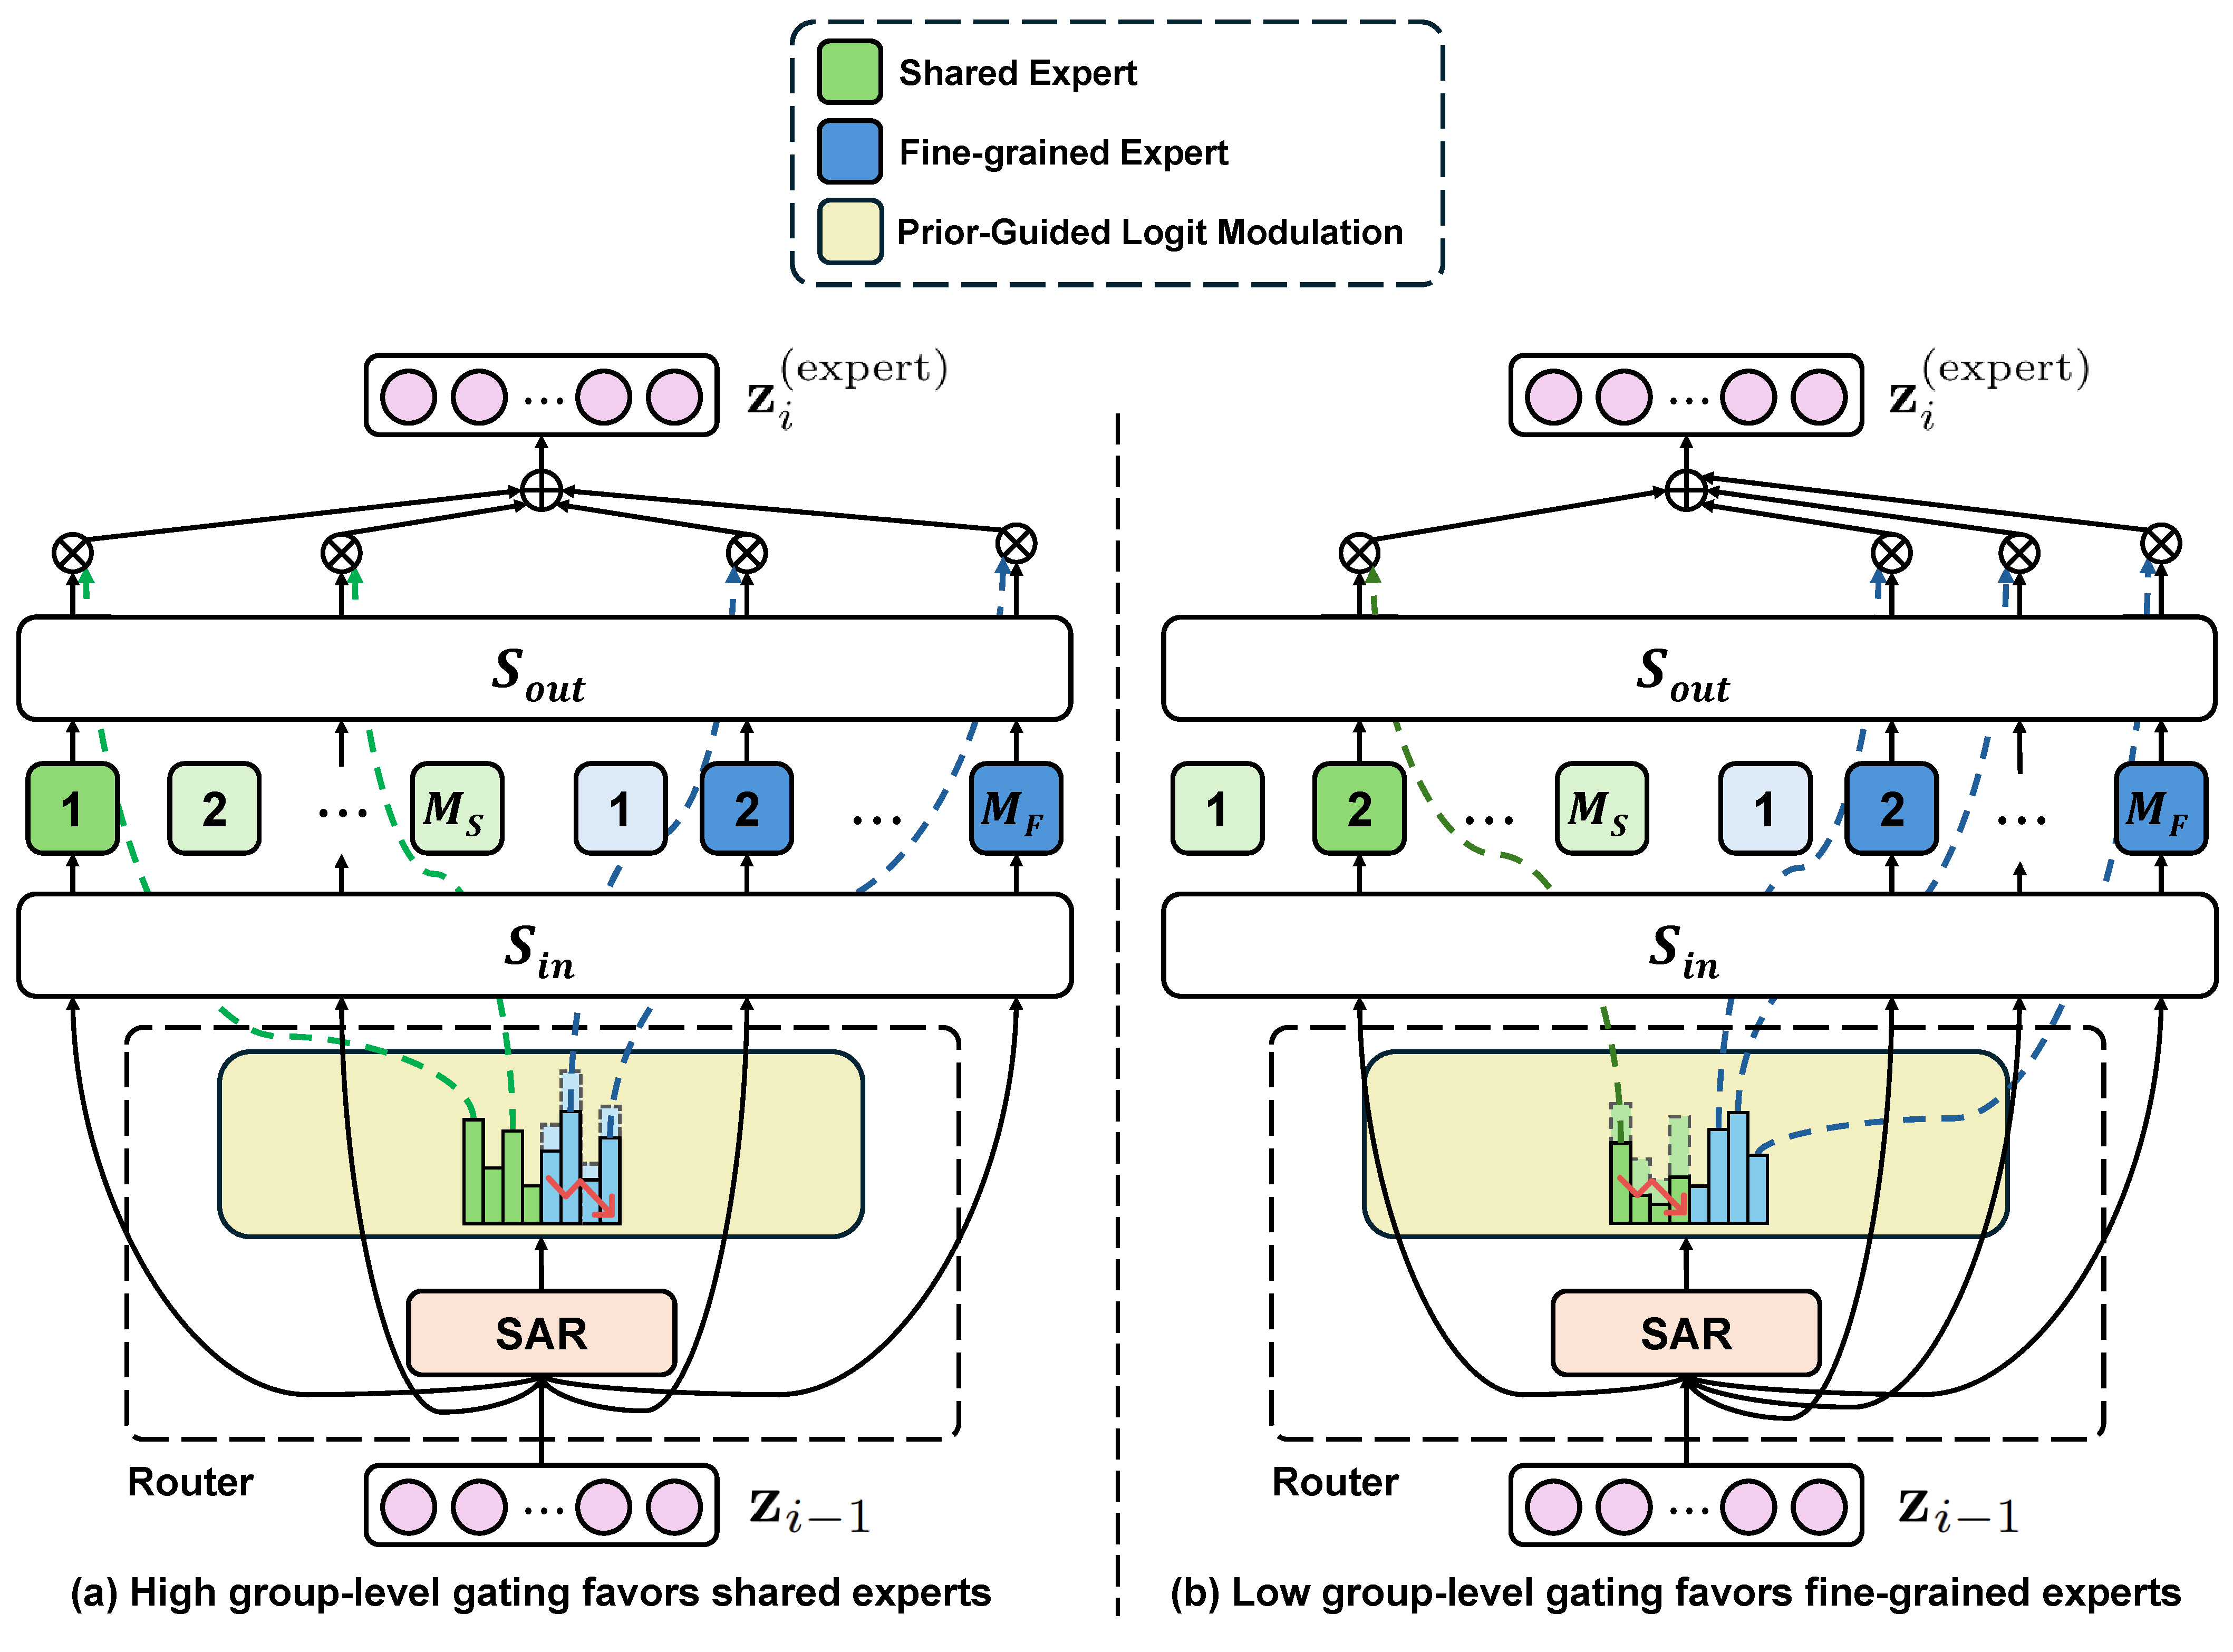
\includegraphics[width=1.0 \linewidth]{figs/router_3.pdf}
    \caption{Hierarchical routing behavior with prior-guided logit modulation (illustrated with Top-$K=4$). \textbf{(a)} For high group gate $g_s$, shared-expert candidates (green) receive a weaker modulation penalty than fine-grained candidates (blue), leading to higher relative rank under Top-$K$ selection. \textbf{(b)} For low $g_s$, the preference is reversed, promoting fine-grained experts for input-specific adaptation. Here, $M_S$ denotes the number of experts in the shared group, $M_F$ denotes the number of experts in the fine-grained group, and the total pool size is $M=M_S+M_F$. Experts shown with darker color fill in the diagram indicate the activated subset. In both regimes, the router computes Semantic Affinity Routing logits, applies group-prior modulation, selects active experts via Top-$K$, and aggregates shape-aligned expert outputs through $S_{\text{in}}$ and $S_{\text{out}}$ into $\mathbf{z}_i^{(\text{expert})}$.}
    \label{fig:sar}
\end{figure}

SAGE employs a two-level routing strategy to construct a sparse, input-dependent expert path while preserving the backbone computation. As illustrated in Figure~\ref{fig:sar}, given a layer input $\mathbf{z}_{i-1}$, the router computes a group-level gate $g_s$, produces base expert logits via Semantic Affinity Routing (SAR), modulates these logits with the group prior, and then performs top-$K$ selection on the modulated logits. This process jointly controls which experts are preferred (shared versus fine-grained) and which experts are finally executed, yielding the sparse expert computation used in Equation~\ref{eq:combination}.



% \vspace{0.1in}

\noindent\textbf{Group-Level Gating.}
A lightweight gating network $G_s$ estimates the group-level preference toward shared experts. It takes a globally pooled representation $\bar{\mathbf{z}}_{i-1} \in \mathbb{R}^d$ and outputs a scalar gate $g_s \in (0,1)$:
\begin{equation}
    g_s = \sigma\left(\bar{\mathbf{z}}_{i-1}\mathbf{W}_{\text{gate}}^{(i)} + b_{\text{gate}}^{(i)}\right).
    \label{eq:gate}
\end{equation}
A high $g_s$ favors shared experts, while a low $g_s$ favors fine-grained experts; shared experts are still selected conditionally via the same top-$K$ routing process.

% \vspace{0.1in}

\noindent\textbf{Semantic Affinity Routing (SAR).}
A primary router $R_i$ computes base logits $\mathbf{L}_i \in \mathbb{R}^{M}$ over all experts $\mathcal{E} = \{E_1, \ldots, E_M\}$:
\begin{equation}
\begin{aligned}
\mathbf{L}_i &= \frac{(\bar{\mathbf{z}}_{i-1}\mathbf{W}_{Q}^{(i)})(\mathbf{K}^{(i)})^{\!\top}}{\sqrt{d_k}} \\
&\quad + \operatorname{softplus}(\bar{\mathbf{z}}_{i-1}\mathbf{W}_{\text{noise}}^{(i)}) \odot \boldsymbol{\epsilon}^{(i)}, \\
\boldsymbol{\epsilon}^{(i)} &\sim \mathcal{N}(\mathbf{0}, \mathbf{I}_M),
\end{aligned}
\label{eq:sar_logits}
\end{equation}
where $\mathbf{W}_{Q}^{(i)} \in \mathbb{R}^{d \times d_k}$ is a learnable query projection, $\mathbf{K}^{(i)} \in \mathbb{R}^{M \times d_k}$ is the expert-key matrix, and $\mathbf{W}_{\text{noise}}^{(i)} \in \mathbb{R}^{d \times M}$ controls input-adaptive noise magnitude. The first term captures semantic affinity, while the second term adds stochastic exploration to improve routing diversity and reduce expert over-specialization. The group-level preference induced by $g_s$ is not applied within SAR; instead, it is introduced afterward via logit modulation.

% \vspace{0.1in}

\noindent\textbf{Prior-Guided Logit Modulation.}
Our hierarchical gating couples \emph{group-level} preference (shared vs. fine-grained experts) with \emph{expert-level} selection. Given the base routing logits $\mathbf{L}_i$ produced by SAR and the scalar shared gate $g_s$, we bias expert scores toward the preferred group before selecting the active experts, without forcing shared experts to remain always active. We define a binary mask $\mathbf{m}_s$, where $(\mathbf{m}_s)_j = 1$ if expert $j \in \mathcal{E}_{\text{shared}}$ and $0$ otherwise. The modulated logits are obtained as:
\begin{equation}
    \mathbf{L}'_i = \mathbf{L}_i + \mathbf{m}_s \log(g_s) + (\mathbf{1} - \mathbf{m}_s) \log(1 - g_s),
    \label{eq:logit_modulation}
\end{equation}
where $\mathbf{1} \in \mathbb{R}^M$ is the all-ones vector. This log-space prior raises shared-expert logits when $g_s$ is high and fine-grained logits when $g_s$ is low. For numerical stability, we clip $g_s$ to $[\epsilon, 1-\epsilon]$, then select $\mathcal{K}=\operatorname{TopKIndices}(\mathbf{L}'_i,K)$. Unlike softmax gating, we use independent sigmoid gates on the selected experts:
\begin{equation}
    w_j = \sigma\big((\mathbf{L}'_i)_j\big) \cdot \mathbf{1}[j \in \mathcal{K}],
    \label{eq:topk_sigmoid}
\end{equation}
where $\sigma(\cdot)$ is the sigmoid function; $\mathbf{w} = \{w_j\}_{j=1}^{M}$. For $k \in \mathcal{K}$, $w_k$ denotes the gate value at expert index $k$. This design permits independent multi-expert activation without simplex normalization across selected experts.


Overall, the integration of logit modulation with top-$K$ sigmoid gating induces a sparse, input-adaptive computation graph that balances efficiency with expert specialization across heterogeneous feature distributions.

\begin{algorithm}[!t]
\caption{\textbf{SAGE Training Algorithm (per mini-batch)}}
\label{alg:sage}
\begin{algorithmic}[1]
\Require Input batch $\mathbf{X}$ with labels $\mathbf{Y}$; model $\mathcal{F}$ with $T$ SAGE layers
\Ensure Total loss $\mathcal{L}_{\text{total}}$ for backpropagation
\State $z_0 \gets \text{Stem}(\mathbf{X})$
\State $\mathcal{L}_{\text{load-balancing}} \gets 0$

\For{$i = 1$ to $T$}
    \State $z_i^{(\text{main})} \gets f_i(z_{i-1})$

    \Statex \textbf{Group-Level Gating and SAR}
    \State $\bar{z}_{i-1} \gets \text{GlobalPool}(z_{i-1})$
    \State $g_s \gets \sigma(\bar{z}_{i-1}\mathbf{W}_{\text{gate}}^{(i)} + b_{\text{gate}}^{(i)})$
    \State $\mathbf{L}_i \gets \text{SAR}(\bar{z}_{i-1})$

    \Statex \textbf{Prior-Guided Logit Modulation}
    \State $g_s \gets \text{clip}(g_s, \epsilon, 1-\epsilon)$
    \State $\mathbf{L}'_i \gets \mathbf{L}_i + \mathbf{m}_s\log(g_s) + (\mathbf{1}-\mathbf{m}_s)\log(1-g_s)$

    \Statex \textbf{Top-$K$ Sigmoid Gating and Expert Execution}
    \State $\mathcal{K} \gets \text{TopKIndices}(\mathbf{L}'_i, K)$
    \State $\mathbf{w}[\mathcal{K}] \gets \sigma(\mathbf{L}'_i[\mathcal{K}]);\; \mathbf{w}[\overline{\mathcal{K}}] \gets 0$
    \State $z_i^{(\text{expert})} \gets 0$
    \For{$k \in \mathcal{K}$}
        \State $\tilde{z}_{i-1}^{(k)} \gets S_{\text{in}}(z_{i-1}, e_k)$
        \State $\hat{z}_i^{(k)} \gets S_{\text{out}}(e_k(\tilde{z}_{i-1}^{(k)}), z_i^{(\text{main})})$
        \State $z_i^{(\text{expert})} \gets z_i^{(\text{expert})} + \mathbf{w}_k\,\hat{z}_i^{(k)}$
    \EndFor

    \State $z_i \gets \alpha_i\,z_i^{(\text{main})} + (1-\alpha_i)\,z_i^{(\text{expert})}$
    \State $\mathcal{L}_{\text{load-balancing}} \gets \mathcal{L}_{\text{load-balancing}} + M\sum_{j=1}^{M} f_j^{(i)}P_j^{(i)}$
\EndFor

\State $\mathbf{P} \gets \text{Decoder}(z_T)$
\State $\mathcal{L}_{\text{task}} \gets \lambda_{\text{ce}}\mathcal{L}_{\text{CE}}(\mathbf{P},\mathbf{Y}) + \lambda_{\text{dice}}\mathcal{L}_{\text{Dice}}(\mathbf{P},\mathbf{Y})$
\State $\mathcal{L}_{\text{total}} \gets \mathcal{L}_{\text{task}} + \lambda_{lb}\mathcal{L}_{\text{load-balancing}}$
\State \Return $\mathcal{L}_{\text{total}}$
\end{algorithmic}
\end{algorithm}

\subsection{Cross-Architecture Adaptation and Fusion}
\label{subsec:sahub}
Executing heterogeneous experts requires resolving representation mismatches between convolutional feature maps $(B,C,H,W)$ and token sequences $(B,N,D)$. We address this with the Shape-Adapting Hub, a lightweight learnable module that performs bidirectional format conversion with explicit shape alignment.

% \vspace{0.1in}

\noindent\textbf{Shape-Adapting Hub (SA-Hub).}
SA-Hub consists of an input adapter $S_{\text{in}}$ and an output adapter $S_{\text{out}}$. For each selected expert $e_k$, we first infer the representation type of the source feature and target expert, then apply a format-aware transformation:
\begin{equation}
    \tilde{\mathbf{z}}_{i-1}^{(k)} = S_{\text{in}}(\mathbf{z}_{i-1}, e_k),
    \label{eq:sahub_in}
\end{equation}
with
\begin{equation*}
S_{\text{in}}(\mathbf{x}, e_k)=
\begin{cases}
\mathcal{A}_{C\rightarrow D}\!\left(\mathcal{F}_{2D\rightarrow 1D}(\mathbf{x})\right),
& \begin{array}[t]{@{}l@{}}
\tau(\mathbf{x})=\text{CNN},\\
\tau(e_k)=\text{Trans.},
\end{array}\\[3pt]
\mathcal{F}_{1D\rightarrow 2D}\!\left(\mathcal{A}_{D\rightarrow C}(\mathbf{x})\right),
& \begin{array}[t]{@{}l@{}}
\tau(\mathbf{x})=\text{Trans.},\\
\tau(e_k)=\text{CNN},
\end{array}\\[3pt]
\mathcal{A}(\mathbf{x}), & \tau(\mathbf{x})=\tau(e_k),
\end{cases}
\end{equation*}
where $\mathcal{F}_{2D\rightarrow 1D}$ flattens spatial maps into token sequences, $\mathcal{F}_{1D\rightarrow 2D}$ reconstructs spatial layout (with interpolation if needed), and $\mathcal{A}$ denotes projections (e.g., $1\times1$ convolution or linear layers) for channel/embedding alignment.

After expert computation, the output adapter maps back to the main-path format with target-shape constraints:
\begin{equation}
    \hat{\mathbf{z}}_i^{(k)} = S_{\text{out}}\bigg(e_k\big(\tilde{\mathbf{z}}_{i-1}^{(k)}\big),\, \mathbf{z}_i^{(\text{main})}\bigg),
    \label{eq:sahub_out}
\end{equation}
where $S_{\text{out}}$ applies the inverse format transformation and enforces the spatial resolution and channel dimensionality of $\mathbf{z}_i^{(\text{main})}$.

Finally, the adapted expert outputs are combined by gating-weighted aggregation:
\begin{equation}
    \mathbf{z}_i^{(\text{expert})} = \sum_{k \in \mathcal{K}} w_k \cdot \hat{\mathbf{z}}_i^{(k)}.
    \label{eq:expert_output}
\end{equation}
This design allows CNN and Transformer experts to be mixed within a routing layer without imposing a shared native tensor format. In implementation, SA-Hub maintains a registry of pre-initialized adapters for common dimensional conversions to reduce runtime overhead while preserving end-to-end differentiability. The complete execution flow of SAGE, including hierarchical gating, shape adaptation, and loss computation, is summarized in Algorithm~\ref{alg:sage}.